\documentclass[12pt,
               a4paper,
               article,
               oneside,
               english,oldfontcommands]{memoir}
\usepackage{student}
% Metadata
\date{\today}
\setmodule{STK3405/4405: Introduction to Risk and Reliability Analysis}
\setterm{Fall, 2023}

%-------------------------------%
% Other details
% TODO: Fill these
%-------------------------------%
\title{Mandatory assingment: 1}
\setmembername{Jonas Semprini Næss}  % Fill group member names

%-------------------------------%
% Add / Delete commands and packages
% TODO: Add / Delete here as you need
%-------------------------------%
\makeatletter
\newcommand*{\rom}[1]{\expandafter\@slowromancap\romannumeral #1@}
\makeatother
%\usepackage[utf8]{inputenc}
\usepackage{setspace}
\usepackage[T1]{fontenc}
\usepackage{titling}% the wheel somebody else kindly made for us earlier
\usepackage{fancyhdr}
\usepackage{fancybox}
\usepackage{epigraph} 
\usepackage{tikz}
\usepackage{bm}
\usepackage{pgfplots}
\pgfplotsset{compat=1.12}
\usepackage{lmodern}
\usepackage{enumitem}
\usepackage{caption}
\usepackage{subcaption}
\usepackage{fancyvrb}
\usepackage[scaled]{beramono}
\usepackage[final]{microtype}
\usepackage{amssymb}
\usepackage{mathtools}
\usepackage{amsthm}
\usepackage{thmtools}
\usepackage{babel}
\usepackage{csquotes}
\usepackage{listings}
\usetikzlibrary{calc,intersections,through,backgrounds}
\usepackage{tkz-euclide} 
\lstset{basicstyle = \ttfamily}
\usepackage{float}
\usepackage{textcomp}
\usepackage{siunitx}
\usepackage{xcolor}
\usepackage{graphicx}
\usepackage[colorlinks, allcolors = uiolink]{hyperref}
\usepackage[noabbrev]{cleveref}
\pretolerance = 2000
\tolerance    = 6000
\hbadness     = 6000
\newcounter{probnum}[section]
\newcounter{subprobnum}[probnum] 
\usepackage{dirtytalk}
\usepackage{listings}
\usepackage{xcolor}
\usepackage{caption}
\usepackage[section]{placeins}
\usepackage{varwidth}
\usepackage{optidef}
\definecolor{uiolink}{HTML}{0B5A9D}
\definecolor{dkgreen}{rgb}{0,0.6,0}
\definecolor{gray}{rgb}{0.5,0.5,0.5}
\definecolor{mauve}{rgb}{0.58,0,0.82}
\lstset{frame=tb,
  language=python,
  aboveskip=3mm,
  belowskip=3mm,
  showstringspaces=false,
  columns=fullflexible,
  basicstyle={\small\ttfamily},
  numbers=none,
  numberstyle=\tiny\color{black},
  keywordstyle=\color{blue},
  commentstyle=\color{dkgreen},
  stringstyle=\color{mauve},
  breaklines=true,
  breakatwhitespace=true,
  tabsize=3} 
\usepackage{commath}
\newtheorem{theorem}{Theorem}[section]
\newtheorem{corollary}{Corollary}[theorem]
\newcommand{\Q}{ \qquad \hfill \blacksquare}
\newcommand\myeq{\stackrel{\mathclap{\normalfont{uif}}}{\sim}}
\let\oldref\ref
\renewcommand{\ref}[1]{(\oldref{#1})}
\newtheorem{lemma}[theorem]{Lemma}
\setlength \epigraphwidth {\linewidth}
\setlength \epigraphrule {0pt}
\AtBeginDocument{\renewcommand {\epigraphflush}{center}}
\renewcommand {\sourceflush} {center}
\parindent 0ex
\renewcommand{\thesection}{\roman{section}} 
\renewcommand{\thesubsection}{\thesection.\roman{subsection}}
\newcommand{\KL}{\mathrm{KL}}
\newcommand{\R}{\mathbb{R}}
\newcommand{\E}{\mathbb{E}}
\newcommand{\T}{\top}
\newcommand{\bl}{\left\{}
\newcommand{\br}{\right\}}
\newcommand{\spaze}{\vspace{4mm}\\}
\newcommand{\N}{\mathbb{N}}
\newcommand{\Rel}{\mathbb{R}}
\newcommand{\expdist}[2]{%
        \normalfont{\textsc{Exp}}(#1, #2)%
    }
\newcommand{\expparam}{\bm \lambda}
\newcommand{\Expparam}{\bm \Lambda}
\newcommand{\natparam}{\bm \eta}
\newcommand{\Natparam}{\bm H}
\newcommand{\sufstat}{\bm u}

% Main document
\begin{document}
\header{}
\section*{\centering Problem 1.}
a.) \emph{Find all the minimal path and cut sets of the system $(C,\phi)$, and determine:}
\begin{align*}
d &= \text{The length of the shortest path} \\[5pt] 
c &= \text{The length of the shortest cut}
\end{align*}
\textbf{Solution:} \spaze
\begin{figure}[H]
\centering 
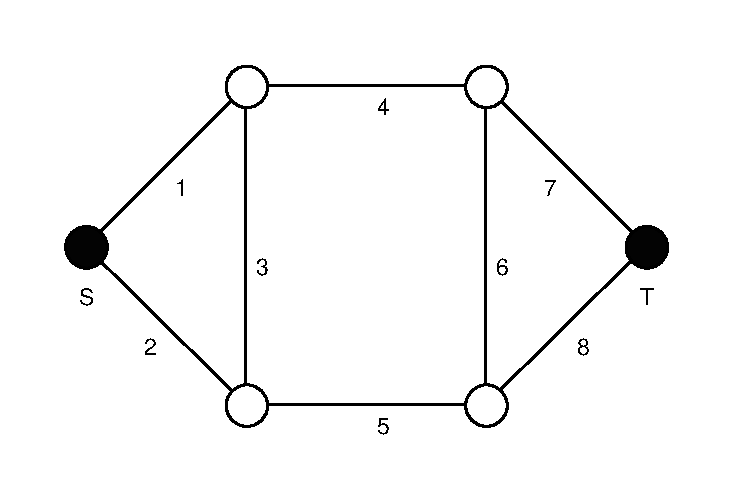
\includegraphics[width=0.7\textwidth]{2-bridge.pdf}
\caption{Visual of the 2-terminal undirected network system}
\end{figure}
We recall that a minimal path set is a path set that cannot be reduced without loosing the validity of being a path set. In this respective example, the following path sets are minimal 
\begin{align*}
P_1 &= \bl 1, 4, 7\br \ P_2 = \bl 2, 5, 8\br  \\[5pt]
P_3 &= \bl 1, 3, 5, 8\br \ P_4 = \bl 2, 5,6,  7\br \ P_5 = \bl 1, 4, 6, 8\br \ P_6 = \bl 2, 3, 4, 7\br  \\[5pt]
P_7 &= \bl 1, 3, 5, 6, 7\br  \ P_8 = \bl 2, 3, 4, 6, 8\br.
\end{align*}
Meaning the 2-terminal system has has two minimal path sets of order 3, four minimal path sets of order 4 and two minimal path sets of order 5. Hence is 
\begin{align*}
d = \min_{P_{i} \in P} |P_{i}|= 3, \quad i = 1, \ldots, 8.
\end{align*}
Next we turn to the cut sets and apply the same reasoning, which yields
\begin{align*}
C_1 &= \bl 1, 2\br \ C_2 = \bl 7, 8 \br  \ C_3 = \bl 4, 5 \br \\[5pt]
C_4 &= \bl 1,3, 5\br \ C_5 = \bl 2,3,4\br  \\[5pt]
C_6 &= \bl 2,5,6, 7\br \ C_7 = \bl 1,4,6, 8\br.
\end{align*}
Thus has the 2-terminal system three minimal cut sets of order 2, two minimal cut sets of order 3, and two minimal cut sets of order 4. Then 
\begin{align*}
d = \min_{C_{j} \in C} |C_{j}|= 2, \quad j = 1, \ldots, 7.
\end{align*}
b.) \emph{Show that the structure function of the system $(C,\phi)$,  can be written as:}
\begin{align*}
\phi(\bm{X}) &= X_3 X_6 \cdot \left( X_1 \coprod X_2 \right) \cdot \left(X_4 \coprod X_5 \right)\cdot \left(X_7 \coprod X_8 \right) \\[5pt]
&+ X_3 (1- X_6) \cdot \left( X_1 \coprod X_2 \right) \cdot \left( \left( X_4 X_7 \coprod X_5 X_8 \right) \right) \\[5pt]
&+ (1 - X_3 )(X_6) \cdot \left( \left(X_1X_4 \coprod X_2 X_5 \right) \right) \cdot \left( X_7 \coprod X_8 \right) \\[5pt]
&+ (1 - X_3 )(1 - X_6) \cdot \left( \left(X_1X_4X_7 \coprod X_2 X_5 X_8 \right) \right)
\end{align*}
\textbf{Solution:} \spaze
To solve this problem we are going to apply pivotal decomposition, and firstly notice that we can write it as follows
\begin{align}
\phi_{1}(\bm{x}) &= x_{i} \phi(1_i, \bm{x}) + (1 - x_{i}) \phi(0_{i}, \bm{x}), \quad i = 1, \ldots, 8 \\[5pt]
\phi_{2}(\bm{x}) &= x_{j} \phi(1_{j}, \bm{x}) + (1 - x_{j}) \phi(0_{j}, \bm{x}), \quad j  = 1, \ldots, 8, \ \neq i
\end{align}
where $\phi(\bm{x})= \phi_{1}(\bm{x}) \cdot \phi_{2}(\bm{x})$ \footnote{Note that this looks very much like module decomposition (even though it is not due to the given sets of states not having an empty intersection), but it was easier to  specify this way.}. Now introduce component three, which gives 
\begin{align*}
\phi_{1}(\bm{X}) &= X_{3} \phi(1_3,  \bm{X}) + (1 - X_3) \phi(0_{3}, \bm{X}) \\[5pt]
&= X_3 \left( X_1 \coprod X_2 \right) \cdot \left(X_4 \coprod X_5 \right) + (1 - X_3)\left(X_1X_4 \coprod X_2 X_5 \right)
\end{align*}
and equally for component six 
\begin{align*}
\phi_{2}(\bm{X}) &= X_{6} \phi(1_6,  \bm{X}) + (1 - X_6) \phi(0_{6}, \bm{X}) \\[5pt]
&= X_6 \left( X_7 \coprod X_8 \right)  + (1 - X_6)\left(X_4X_7 \coprod X_5 X_8 \right)
\end{align*}
Where we neglect the $\left(X_4 \coprod X_5 \right) $ term due to redundancy on the system state. Hence do we have that 
\begin{align*}
\phi(\bm{x}) &= X_3 \left( X_1 \coprod X_2 \right) \cdot \left(X_4 \coprod X_5 \right) + (1 - X_3)\left(X_1X_4 \coprod X_2 X_5 \right) \\[8pt]
&\cdot \left( X_6 \left( X_7 \coprod X_8 \right)  + (1 - X_6)\left(X_4X_7 \coprod X_5 X_8 \right) \right) \\[8pt]
&= X_3X_6 \left( X_1 \coprod X_2 \right) \cdot \left(X_4 \coprod X_5 \right) \cdot\left( X_7 \coprod X_8 \right) \\[8pt] 
&+ X_3(1-X_6) \cdot \left( X_1 \coprod X_2 \right) \cdot \left( \left( X_4 X_7 \coprod X_5 X_8 \right) \right) \\[8pt]
&+ (1 - X_3 )(X_6) \cdot \left( \left(X_1X_4 \coprod X_2 X_5 \right) \right) \cdot \left( X_7 \coprod X_8 \right) \\[8pt]
&+ (1 - X_3 )(1 - X_6)  \left(X_1X_4 \coprod X_2 X_5 \right)\left(X_4X_7 \coprod X_5 X_8 \right)
\end{align*}
where $\left(X_1X_4 \coprod X_2 X_5 \right) \cdot \left(X_4X_7 \coprod X_5 X_8 \right) =  \left(X_1X_4X_7 \coprod X_2 X_5 X_8 \right) $, since $X_1, X_4, X_7$ and $X_2, X_5, X_8$ are in respective series systems when component three and six are not working. Thus is 
\begin{align*}
\phi(\bm{X}) &= X_3 X_6 \cdot \left( X_1 \coprod X_2 \right) \cdot \left(X_4 \coprod X_5 \right)\cdot \left(X_7 \coprod X_8 \right) \\[5pt]
&+ X_3 (1- X_6) \cdot \left( X_1 \coprod X_2 \right) \cdot \left( \left( X_4 X_7 \coprod X_5 X_8 \right) \right) \\[5pt]
&+ (1 - X_3 )(X_6) \cdot \left( \left(X_1X_4 \coprod X_2 X_5 \right) \right) \cdot \left( X_7 \coprod X_8 \right) \\[5pt]
&+ (1 - X_3 )(1 - X_6) \cdot \left( \left(X_1X_4X_7 \coprod X_2 X_5 X_8 \right) \right).
\end{align*}
And we are done. $\Q$ \spaze
c.) \emph{Use the result from (b) to find a similar expression for:}
\begin{align*}
h(\bm{p}) = P(\phi(\bm{X}) = 1) = E[\phi(\bm{X})]
\end{align*}
\textbf{Solution:}\spaze 
The reliability of a binary monotone system we remember is defined as the probability that the system is functioning, which more broadly can be described as 
\begin{align*}
h = \mathbb{E}[\phi(\bm{X})] = \sum_{x \in \bl 0,1 \br^n} \phi(\bm{X})\mathbb{P}( \bm{X} = \bm{x}).
\end{align*}
This implies that are we able, in like manner, as for the structure function, to calculate the reliability of $\phi(\bm{X})$ to be 
\begin{align*}
h(\bm{p}) &= p_3 p_6 \cdot \left( p_1 \coprod p_2 \right) \cdot \left(p_4 \coprod p_5 \right)\cdot \left(p_7 \coprod p_8 \right) \\[5pt]
&+ p_3 (1- p_6) \cdot \left( p_1 \coprod p_2 \right) \cdot \left( \left( p_4 p_7 \coprod p_5 p_8 \right) \right) \\[5pt]
&+ (1 - p_3 )(p_6) \cdot \left( \left(p_1p_4 \coprod p_2 p_5 \right) \right) \cdot \left( p_7 \coprod p_8 \right) \\[5pt]
&+ (1 - p_3 )(1 - p_6) \cdot \left( \left(p_1p_4p_7 \coprod p_2 p_5 p_8 \right) \right).
\end{align*}
d.) \emph{The modified script should calculate the true reliability of the system using the expression for the reliability function $h(\bm{p})$ derived in (c), and also estimate this reliability based on the simulation results. Finally, the script should create a plot of the convergence curve described above and save this in a file in a folder called crudegen.} \spaze 
\textbf{Solution:} \spaze 
When running the implemented code (\ref{lst:crude rel}) using crude Monte Carlo simulations, we obtain the following plot 
\begin{figure}[H]
\centering 
\includegraphics[width=0.8\textwidth]{crudegen/bridge.pdf}
\caption{Plot showing the 1000 crude Monte Carlo simulations, and the corresponding estimate it produces (i.e red curve)}
\end{figure}
with the following estimate 
\begin{table}[H] 
  \begin{center} 
    \label{tab:c mont rel}
    \begin{tabular}{c c} 
      \textbf{Actual:} $h$ & \textbf{Estimated}: $\hat{h}$ \\
      \hline
       0.106272 &  0.103 \\
      \hline 
    \end{tabular}
     \caption{Values of true reliability against the estimated Monte Carlo reliability}
  \end{center}
\end{table}
e.) \emph{Assuming that $\hat{\theta}_0 , \hat{\theta}_1, \ldots, \hat{\theta}_8$ are unbiased estimates i.e $E[\hat{\theta}_s ]= \theta_s$, $s=0, 1, \ldots, 8$ show that}
\begin{align*}
E(\hat{h}_{CMC}) = h
\end{align*}
\textbf{Solution:} \spaze 
By definiton we know that the estimated reliability doing conditional Monte Carlo simulations is 
\begin{align*}
\hat{h}_{CMC} = \sum_{s=0}^{8} \hat{\theta}_s \mathbb{P}( S = s)
\end{align*}
which if we write out the sum gives 
\begin{align*}
\hat{h}_{CMC} = \hat{\theta}_0\mathbb{P}( S = 0) +  \hat{\theta}_1\mathbb{P}( S = 1) + \cdots +  \hat{\theta}_8\mathbb{P}( S = 8).
\end{align*}
Then we take the expected value of the sum 
\begin{align*}
\mathbb{E}  \left[\sum_{s=0}^{8} \hat{\theta}_s \mathbb{P}( S = s) \right] = \mathbb{E} \left[ \hat{\theta}_0\mathbb{P}( S = 0) \right] + \mathbb{E} \left[ \hat{\theta}_1\mathbb{P}( S = 1) \right] + \cdots + \mathbb{E} \left[ \hat{\theta}_8\mathbb{P}( S = 8) \right]
\end{align*}
and apply the fact that $\hat{\theta}_0 , \hat{\theta}_1, \ldots, \hat{\theta}_8$ are unbiased estimates 
\begin{align*}
\mathbb{E}  \left[\sum_{s=0}^{8} \hat{\theta}_s \mathbb{P}( S = s) \right] &= \mathbb{E} \left[ \theta_0\mathbb{P}( S = 0) \right] + \mathbb{E} \left[ \theta_1\mathbb{P}( S = 1) \right] + \cdots + \mathbb{E} \left[ \theta_8 \mathbb{P}( S = 8) \right] \\[5pt]
&= \sum_{s=0}^{8} \theta_s \mathbb{P}( S = s) \\[5pt]
&= h
\end{align*}
and we are done. $\Q$ \spaze
f.) \emph{Explain why $ \theta_0 = \theta_1 = \theta_2 = 0$, while $\theta_7 = \theta_8 = 1.$ How can this be used to make the conditional simulations more efficient?} \spaze 
\textbf{Solution:} \spaze 
When running conditional Monte Carlo simulations we would like to minimise the variance of the estimate we are making as much as possible. This can be done thorugh constructing $S$ in such a way that it contains as much information about $\phi$ as possible. This means that in the process we only calculate the conditional probabilities we really need, and can only cost us a time complexity of $\mathcal{O}(n)$. Nonetheless, is it possible to improve the time complexity further when applying specified focus and precision on the estimates that affect the simulations the most. \vspace{2mm} \\
We recall the results in (a.) found through the minimal path and cut sets, and observe in relation to the Monte Carlo simulations that it is superflous to spend time on estimating any $\hat{\theta}_s, \ s < d \ \lor s > n - c$ since these estimates are more or less deterministic already. \vspace{2mm}\\
Hence in summary, is it beneficial to let
\begin{align*}
	\begin{cases}
		\hat{\theta}_s = 0, &  s < d \\[5pt] 
		\hat{\theta}_s = 1, & s > n - c
	\end{cases}
\end{align*}
where $n$ is the number of components. This then says that in our example
\begin{align*}
\begin{cases}
		\hat{\theta}_s = 0, &  s < 3 \\[5pt] 
		\hat{\theta}_s = 1, & s > 6
 \end{cases}
\end{align*}
which is what we wanted to show. $\Q$ \spaze
g.) \emph{The modified script should calculate the distribution of the variable S defined above, and estimate the conditional expectations $\theta_3, \ldots, \theta_6$. Moreover, the script should calculate the true reliability of the system using the expression for the reliability function $h(p)$ derived in (c), and also estimate this reliability based on the simulation results. Finally, the script should create a plot of the convergence curve described above and save this in a file in a folder called cmcgen.} \spaze
\textbf{Solution:} \spaze 
The code showcased in (\ref{lst:cond rel}) produces the follwing plot and results 
\begin{figure}[H]
\centering 
\includegraphics[width=0.7\textwidth]{cmcgen/bridge.pdf}
\caption{Plot showing the 1000 conditional Monte Carlo simulations, and the corresponding estimate it produces (i.e red curve)}
\end{figure}
\begin{table}[H] 
  \begin{center} 
    \label{tab:con mont}
    \begin{tabular}{c c} 
       $\mathbb{P}(S = s)$ & Probability\\
      \hline
     $\mathbb{P}(S = 1)$ & 0.003528\\
	 $\mathbb{P}(S = 2)$ & 0.031248000000000005\\
	 $\mathbb{P}(S = 3)$  & 0.11588200000000001\\
	 $\mathbb{P}(S = 4)$& 0.23502200000000006\\
	 $\mathbb{P}(S = 5)$& 0.28492000000000006\\
	 $\mathbb{P}(S = 5)$ & 0.211212\\
	 $\mathbb{P}(S = 6)$ & 0.093402\\
	 $\mathbb{P}(S = 7)$ &0.022518000000000003\\
	 $\mathbb{P}(S = 8)$ & 0.002268 \\
      \hline 
    \end{tabular}
     \caption{Distribution of probability values for $S$}
  \end{center}
\end{table}
\begin{table}[H] 
  \begin{center} 
    \label{tab:theta_1}
    \begin{tabular}{c c} 
       $\theta_s$ & Estimate\\
      \hline
$\theta_3$ & 0.0\\
$\theta_4 $ & 0.0\\
$\theta_5$ & 0.19047619047619047\\
$\theta_6$ & 0.5321100917431193\\
      \hline 
    \end{tabular}
     \caption{Estimate values of $\theta_s$ for  $s = 3, 4, 5, 6$}
  \end{center}
\end{table}
\begin{table}[H] 
  \begin{center} 
    \label{tab:con mont rel}
    \begin{tabular}{c c} 
      \textbf{Actual:} $h$ & \textbf{Estimated}: $\hat{h}$ \\
      \hline
      0.106272 &  0.11471700393184797\\
      \hline 
    \end{tabular}
     \caption{Values of true reliability against the estimated Monte Carlo reliability}
  \end{center}
\end{table}
Where we observe that the estimate for $\hat{h}$ is actually worse for conditioned Monte Carlo simulations (although very slighty). Why this is so might vary, but logically it might have to with the fact that our system is not particulalry large in size (number of components), hence short paths to estimate, whereas the Monte Carlo simulations might not accurately enough capture the conditional relationships. \spaze 
h.) \emph{By using the result from (c) show that:}
\begin{align*}
h(p) &= p^2 \cdot \left( p \coprod p \right) \cdot  \left( p \coprod p \right) \cdot  \left( p \coprod p \right) \\[5pt]
&+ 2p(1-p) \cdot \left( p \coprod p \right) \cdot \left( p^2 \coprod p^2 \right) \\[5pt]
&+ (1-p)^2 \cdot \left( p^3 \coprod p^3 \right)
\end{align*}
\textbf{Solution:} \spaze 
From (c.) we had that 
\begin{align*}
h(\bm{p}) &= p_3 p_6 \cdot \left( p_1 \coprod p_2 \right) \cdot \left(p_4 \coprod p_5 \right)\cdot \left(p_7 \coprod p_8 \right) \\[5pt]
&+ p_3 (1- p_6) \cdot \left( p_1 \coprod p_2 \right) \cdot \left( \left( p_4 p_7 \coprod p_5 p_8 \right) \right) \\[5pt]
&+ (1 - p_3 )(p_6) \cdot \left( \left(p_1p_4 \coprod p_2 p_5 \right) \right) \cdot \left( p_7 \coprod p_8 \right) \\[5pt]
&+ (1 - p_3 )(1 - p_6) \cdot \left( \left(p_1p_4p_7 \coprod p_2 p_5 p_8 \right) \right).
\end{align*}
where if we plug in that all probabilities are equal gives 
\begin{align}
h(p) &= p \cdot p \cdot \left( p \coprod p \right) \cdot \left(p \coprod p \right) \cdot \left(p \coprod p \right) \\[5pt]
&+ p (1- p) \cdot \left( p \coprod p \right) \cdot \left( \left( p\cdot p \coprod p \cdot p \right) \right) \\[5pt]
&+ (1 - p )(p) \cdot \left( \left(p \cdot p \coprod p \cdot p \right) \right) \cdot \left( p \coprod p \right) \\[5pt]
&+ (1 - p )(1 - p) \cdot \left( \left(p \cdot p \cdot p \coprod p \cdot p \cdot p \right) \right).
\end{align}
which is nothing more than 
\begin{align*}
h(p) &= p^2 \cdot \left( p \coprod p \right) \cdot  \left( p \coprod p \right) \cdot  \left( p \coprod p \right) \\[5pt]
&+ 2p(1-p) \cdot \left( p \coprod p \right) \cdot \left( p^2 \coprod p^2 \right) \\[5pt]
&+ (1-p)^2 \cdot \left( p^3 \coprod p^3 \right)
\end{align*}
when observing that (4) ad (5) are the same expression. $\Q$ \spaze 
i.) \emph{The modified script should create a plot containing both the true reliability function, as well as the estimated reliability function based on the simulation results, and save this in a file in a folder called crude.} \spaze 
\textbf{Solution:} \spaze 
By code  (\ref{lst:crude rel prob}) we obtain the followig plot 
\begin{figure}[H]
\centering 
\includegraphics[width=0.7\textwidth]{crude/bridge.pdf}
\caption{Plot showing the 1000 crude Monte Carlo simulations for equal probabilities, and the corresponding estimate it produces (i.e red curve)}
\end{figure}
j.) \emph{The modified script should create a plot containing both the true reliability function, as well as the estimated reliability function based on the simulation results, and save this in a file in a folder called cmc.} \spaze
\textbf{Solution:} \spaze 
The script at (\ref{lst:cond rel prob}) produces the following plot and result 
\begin{figure}[H]
\centering 
\includegraphics[width=0.7\textwidth]{cmc/bridge.pdf}
\caption{Plot showing the 1000 conditional Monte Carlo simulations for equal probabilities, and the corresponding estimate it produces (i.e red curve)}
\end{figure}
\begin{table}[H] 
  \begin{center} 
    \label{tab:con mont prob}
    \begin{tabular}{c c} 
      $\hat{\theta}_s$ & \textbf{Estimation} \\
      \hline
     	$\hat{\theta}_0 $ &  0 \\
     	$\hat{\theta}_1 $ & 0 \\
     	$\hat{\theta}_2 $ & 0 \\
     	$\hat{\theta}_3 $ & 0 \\
     	$\hat{\theta}_4 $ & 0 \\
     	$\hat{\theta}_5 $ & 0.146 \\
     	$\hat{\theta}_6 $ & 0.438 \\
     	$\hat{\theta}_7 $ & 0.721\\
     	$\hat{\theta}_8 $ & 1\\
      \hline 
    \end{tabular}
     \caption{Values of true reliability against the estimated Monte Carlo reliability}
  \end{center}
\end{table}
which by clear observation is an even better and more accurate estimation of $h$ than the crude Monte Carlo method provides (though still only minor differences). \vspace{2mm}\\ 
Now seeing as the probabilities are equal the conditional Monte Carlo excels due to  its employment of conditional information. Since the probabilities are equal they now become dependent and thus can cause an increase in variance, which conditional Monte Carlo simulations deal with more adeptly than the crude simulations.
\section*{\centering \underline{Appendix}}
\subsubsection*{\centering Source code}
\begin{lstlisting}[caption= Crude Monte Carlo Reliability (exercise d.), label={lst:crude rel}]
import matplotlib.pyplot as plt
import numpy as np

plt.style.use("Solarize_Light2")
# Number of simulations
num_sims = 1000

# Interval between h_hat calculations
h_interv = 10

# Random number generator seed. Set to 'None' for a random sequence
seed_num = 1234
gen = np.random.default_rng(seed=seed_num)

# Save plot to file or not?
save_plot = True

# Name of system
sys_name = "bridge"

# Number of components:
n = 8

# Component reliabilities
px = [
    0.0,
    0.6,
    0.3,
    0.5,
    0.4,
    0.7,
    0.5,
    0.3,
    0.6,
]  # P(X_i = px[i]), i = 1, .., n. px[0] is not used


def coprod(x, y):
    return x + y - x * y


def phi(xx):
    system = (
        xx[3]
        * xx[6]
        * coprod(xx[1], xx[2])
        * coprod(xx[4], xx[5])
        * coprod(xx[7], xx[8])
    )

    +((1 - xx[3]) * xx[6] * coprod(xx[1] * xx[4], xx[2] * xx[5]) * coprod(xx[7], xx[8]))

    +((1 - xx[6]) * xx[3] * coprod(xx[1], xx[2]) * coprod(xx[4] * xx[7], xx[5] * xx[8]))

    +((1 - xx[3]) * (1 - xx[6]) * coprod(xx[1] * xx[4] * xx[7], xx[2] * xx[5] * xx[8]))
    return system


def hh(pp):
    rel = (
        pp[3]
        * pp[6]
        * coprod(pp[1], pp[2])
        * coprod(pp[4], pp[5])
        * coprod(pp[7], pp[8])
    )

    +((1 - pp[3]) * pp[6] * coprod(pp[1] * pp[4], pp[2] * pp[5]) * coprod(pp[7], pp[8]))

    +((1 - pp[6]) * pp[3] * coprod(pp[1], pp[2]) * coprod(pp[4] * pp[7], pp[5] * pp[8]))

    +((1 - pp[3]) * (1 - pp[6]) * coprod(pp[1] * pp[4] * pp[7], pp[2] * pp[5] * pp[8]))
    return rel


X = np.zeros(n + 1, dtype=int)  # The component state variables (X[0] is not used)

I = []
H = []
H_hat = []
T = 0

# Calculate the true system reliability
h = hh(px)

for sim in range(num_sims):
    U = gen.uniform(0.0, 1.0, n + 1)  # Uniform variables (U[0] is not used)
    for m in range(1, n + 1):
        if U[m] <= px[m]:
            X[m] = 1
        else:
            X[m] = 0
    T += phi(X)
    if sim > 0 and sim % h_interv == 0:
        h_hat = T / sim
        I.append(sim)
        H.append(h)
        H_hat.append(h_hat)

# Estimate final system reliability
h_hat = T / num_sims

print("h = ", h, ", h_hat = ", h_hat)

plt.plot(I, H, "b", label="True h")
plt.plot(I, H_hat, "r", label="h_hat(iteration)")

plt.ylim(h - 0.2, h + 0.2)
plt.xlabel("iteration")
plt.ylabel("h")

plt.title("Convergence curve for " + sys_name + " system")
plt.legend()
if save_plot:
    plt.savefig("crudegen/" + sys_name + ".pdf")
plt.show()
\end{lstlisting}

\begin{lstlisting}[caption= Conditional Monte Carlo Reliability (exercise g.), label={lst:cond rel}]
import matplotlib.pyplot as plt
import numpy as np

plt.style.use("Solarize_Light2")

# Number of simulations
num_sims = 1000

# Interval between h_hat calculations
h_interv = 10

# Random number generator seed. Set to 'None' for a random sequence
seed_num = 1234
gen = np.random.default_rng(seed=seed_num)

# Save plot to file or not?
save_plot = True

# Name of system
sys_name = "bridge"

# Number of components:
n = 8

# Length of shortest path
d = 3

# Length of shortest cut
c = 2

# Component reliabilities
px = [
    0,
    0.6,
    0.3,
    0.5,
    0.4,
    0.7,
    0.5,
    0.3,
    0.6,
]  # P(X_i = px[i]), i = 1, .., n. px[0] is not used


def coprod(x, y):
    return x + y - x * y


def phi(xx):
    system = (
        xx[3]
        * xx[6]
        * coprod(xx[1], xx[2])
        * coprod(xx[4], xx[5])
        * coprod(xx[7], xx[8])
    )

    +((1 - xx[3]) * xx[6] * coprod(xx[1] * xx[4], xx[2] * xx[5]) * coprod(xx[7], xx[8]))

    +((1 - xx[6]) * xx[3] * coprod(xx[1], xx[2]) * coprod(xx[4] * xx[7], xx[5] * xx[8]))

    +((1 - xx[3]) * (1 - xx[6]) * coprod(xx[1] * xx[4] * xx[7], xx[2] * xx[5] * xx[8]))
    return system


def hh(pp):
    rel = (
        pp[3]
        * pp[6]
        * coprod(pp[1], pp[2])
        * coprod(pp[4], pp[5])
        * coprod(pp[7], pp[8])
    )

    +((1 - pp[3]) * pp[6] * coprod(pp[1] * pp[4], pp[2] * pp[5]) * coprod(pp[7], pp[8]))

    +((1 - pp[6]) * pp[3] * coprod(pp[1], pp[2]) * coprod(pp[4] * pp[7], pp[5] * pp[8]))

    +((1 - pp[3]) * (1 - pp[6]) * coprod(pp[1] * pp[4] * pp[7], pp[2] * pp[5] * pp[8]))
    return rel


# Compute the distributions of S_1, ... , S_n, where S_m = X_m + ... + X_n, m = 1, ..., n
ps = np.zeros(
    [n + 1, n + 1]
)  # P(S_m = s) = ps[m,s], s = 0, 1, ..., (n-m+1). ps[0,s] is not used

ps[n, 0] = 1.0 - px[n]  # P(S_n = 0) = 1 - P(X_n = 1)
ps[n, 1] = px[n]  # P(S_n = 1) = P(X_n = 1)

for j in range(1, n):
    m = n - j
    ps[m, 0] = ps[m + 1, 0] * (1.0 - px[m])  # P(S_m = 0) = P(S_{m+1} = 0) * P(X_m = 0)

    for s in range(1, n - m + 1):
        ps[m, s] = ps[m + 1, s - 1] * px[m] + ps[m + 1, s] * (
            1.0 - px[m]
        )  # P(S_m = s) = P(S_{m+1} = s-1) * P(X_m = 1)
        # + P(S_{m+1} = s) * P(X_m = 0)

    ps[m, n - m + 1] = (
        ps[m + 1, n - m] * px[m]
    )  # P(S_m = n-m+1) = P(S_{m+1} = n-m) * P(X_m = 1)

# Print the distribution of S = S_1
for s in range(n + 1):
    print("P(S = " + str(s) + ") =", ps[1, s])

# Calculate pdc = P(d <= S_1 <= n-c)
pdc = 0
for s in range(d, n - c + 1):
    pdc += ps[1, s]

# Calculate pcn = P(n-c < S_1 <= n)
pcn = 0
for s in range(n - c + 1, n + 1):
    pcn += ps[1, s]


# Sample S_1 from the set {d, ... , n-c}
def sampleS():
    u = gen.uniform(0.0, pdc)
    for s in range(d, n - c):
        if u < ps[1, s]:
            return s
        else:
            u -= ps[1, s]
    return n - c


X = np.zeros(n + 1, dtype=int)  # The component state variables (X[0] is not used)
T = np.zeros(
    n + 1, dtype=int
)  # T[s] counts random path sets of size s = d, 1, ..., n-c
V = np.zeros(n + 1, dtype=int)  # V[s] counts random sets of size s = d, 1, ..., n-c

I = []
H = []
H_hat = []

# Calculate the true system reliability
h = hh(px)

# Run the simulations
for sim in range(num_sims):
    s = sampleS()
    V[s] += 1
    U = gen.uniform(0.0, 1.0, n + 1)  # Uniform variables (U[0] is not used)
    sumx = 0
    for m in range(1, n):
        if sumx < s:
            p = px[m] * ps[m + 1, s - sumx - 1] / ps[m, s - sumx]
            if U[m] <= p:
                X[m] = 1
            else:
                X[m] = 0
            sumx += X[m]
        else:
            X[m] = 0
    if sumx < s:
        X[n] = 1
    else:
        X[n] = 0
    T[s] += phi(X)
    if sim > 0 and sim % h_interv == 0:
        h_hat = pcn
        for s in range(d, n - c + 1):
            if V[s] > 0:
                h_hat += ps[1, s] * T[s] / V[s]
        I.append(sim)
        H.append(h)
        H_hat.append(h_hat)

# Print the estimated conditional reliabilities, theta_s, s = d, ..., n-c
for s in range(d, n - c + 1):
    print("theta_" + str(s) + " =", T[s] / V[s])

# Estimate final system reliability
h_hat = pcn

for s in range(d, n - c + 1):
    h_hat += ps[1, s] * T[s] / V[s]

print("h = ", h, ", h_hat = ", h_hat)

plt.plot(I, H, color="blue", label="True h")
plt.plot(I, H_hat, color="red", label="h_hat(iteration)")
plt.ylim(h - 0.2, h + 0.2)
plt.xlabel("iteration")
plt.ylabel("h")
plt.title("Convergence curve for " + sys_name + " system")
plt.legend()
if save_plot:
    plt.savefig("cmcgen/" + sys_name + ".pdf")
plt.show()
\end{lstlisting}
\begin{lstlisting}[caption= Crude Monte Carlo Reliability (exercise i.), label={lst:crude rel prob}]
import matplotlib.pyplot as plt
import numpy as np

plt.style.use("Solarize_Light2")
# Number of simulations
num_sims = 1000

# Random number generator seed. Set to 'None' for a random sequence
seed_num = 1234
gen = np.random.default_rng(seed=seed_num)

# Number of points
num_points = 101

# Save plot to file or not?
save_plot = True

# Name of system
sys_name = "bridge"

# Number of components:
n = 8


def coprod(x, y):
    return x + y - x * y


def phi(xx):
    system = (
        xx[3]
        * xx[6]
        * coprod(xx[1], xx[2])
        * coprod(xx[4], xx[5])
        * coprod(xx[7], xx[8])
    )

    +((1 - xx[3]) * xx[6] * coprod(xx[1] * xx[4], xx[2] * xx[5]) * coprod(xx[7], xx[8]))

    +((1 - xx[6]) * xx[3] * coprod(xx[1], xx[2]) * coprod(xx[4] * xx[7], xx[5] * xx[8]))

    +((1 - xx[3]) * (1 - xx[6]) * coprod(xx[1] * xx[4] * xx[7], xx[2] * xx[5] * xx[8]))
    return system


def hh(pp):
    rel = pp**2 * coprod(pp, pp) * coprod(pp, pp) * coprod(pp, pp)

    +(2 * pp * (1 - pp) * coprod(pp**2, pp**2) * coprod(pp, pp))

    +((1 - pp) ** 2 * coprod(pp**3, pp**3))
    return rel


X = np.zeros(n + 1, dtype=int)  # The component state variables (X[0] is not used)

p = np.linspace(0, 1, num_points)
T = np.zeros(num_points, dtype=int)

for _ in range(num_sims):
    U = gen.uniform(0.0, 1.0, n + 1)  # Uniform variables (U[0] is not used)
    for j in range(num_points):
        for i in range(1, n + 1):
            if U[i] <= p[j]:
                X[i] = 1
            else:
                X[i] = 0
        T[j] += phi(X)

h_hat = [T[i] / num_sims for i in range(num_points)]

h = np.zeros(num_points)  # True reliability function

for j in range(num_points):
    h[j] = hh(p[j])


plt.plot(p, h, color="blue", label="h(p)")
plt.plot(p, h_hat, color="red", label="h_hat(p)")
plt.xlabel("p")
plt.ylabel("h")
plt.title("Reliability function of " + sys_name + " system")
plt.legend()
if save_plot:
    plt.savefig("crude/" + sys_name + ".pdf")
plt.show()
\end{lstlisting}
\begin{lstlisting}[caption= Conditional Monte Carlo Reliability (exercise j.), label={lst:cond rel prob}]
from scipy.stats import binom
import matplotlib.pyplot as plt
import numpy as np

plt.style.use("Solarize_Light2")
# Number of simulations
num_sims = 1000

# Random number generator seed. Set to 'None' for a random sequence
seed_num = 1234
gen = np.random.default_rng(seed=seed_num)

# Number of points
num_points = 101

# Save plot to file or not?
save_plot = True

# Name of system
sys_name = "bridge"

# Number of components:
n = 8


def coprod(x, y):
    return x + y - x * y


def phi(xx):
    system = (
        xx[3]
        * xx[6]
        * coprod(xx[1], xx[2])
        * coprod(xx[4], xx[5])
        * coprod(xx[7], xx[8])
    )

    +((1 - xx[3]) * xx[6] * coprod(xx[1] * xx[4], xx[2] * xx[5]) * coprod(xx[7], xx[8]))

    +((1 - xx[6]) * xx[3] * coprod(xx[1], xx[2]) * coprod(xx[4] * xx[7], xx[5] * xx[8]))

    +((1 - xx[3]) * (1 - xx[6]) * coprod(xx[1] * xx[4] * xx[7], xx[2] * xx[5] * xx[8]))
    return system


def hh(pp):
    rel = pp**2 * coprod(pp, pp) * coprod(pp, pp) * coprod(pp, pp)

    +(2 * pp * (1 - pp) * coprod(pp**2, pp**2) * coprod(pp, pp))

    +((1 - pp) ** 2 * coprod(pp**3, pp**3))
    return rel


C = list(range(1, n + 1))  # The component set [1, 2, ..., n]
X = np.zeros(n + 1, dtype=int)  # The component state variables (X[0] is not used)
T = np.zeros(
    n + 1, dtype=int
)  # T[s] counts the number of random path sets of size s = 0, 1, ..., n

for _ in range(num_sims):
    for i in range(1, n + 1):
        X[i] = 0
    sys_state = phi(
        X
    )  # phi(0,...0) will always be zero unless we have a trivial system
    T[0] += sys_state
    gen.shuffle(C)  # Generate a random permutation of the component set C
    for i in range(1, n + 1):
        X[C[i - 1]] = 1
        if (
            sys_state == 0
        ):  # If sys_state = 1 already, we know phi(X) = 1 since phi is non-decreasing
            sys_state = phi(X)
        T[i] += sys_state

s_values = list(range(n + 1))  # Set of possible values of S = X[1] + ... + X[n]

theta_hat = [
    T[s] / num_sims for s in s_values
]  # theta_hat[s] = Estimated conditional reliability given S = s
print(theta_hat)

p = np.linspace(0, 1, num_points)
h = np.zeros(num_points)  # True reliability function
h_hat = np.zeros(num_points)  # Estimated reliability function
for j in range(num_points):
    h[j] = hh(p[j])
    dist = [binom.pmf(s, n, p[j]) for s in s_values]
    for s in range(n + 1):
        h_hat[j] += theta_hat[s] * dist[s]

plt.plot(p, h, color="blue", label="h(p)")
plt.plot(p, h_hat, color="red", label="h_hat(p)")
plt.xlabel("p")
plt.ylabel("h")
plt.title("Reliability function of " + sys_name + " system")
plt.legend()
if save_plot:
    plt.savefig("cmc/" + sys_name + ".pdf")
plt.show()
\end{lstlisting} 
\end{document}